%%%%%%%%%%%%%%%%%%%%%%% file template.tex %%%%%%%%%%%%%%%%%%%%%%%%%
%
% This is a general template file for the LaTeX package SVJour3
% for Springer journals.          Springer Heidelberg 2010/09/16
%
% Copy it to a new file with a new name and use it as the basis
% for your article. Delete % signs as needed.
%
% This template includes a few options for different layouts and
% content for various journals. Please consult a previous issue of
% your journal as needed.
%
%%%%%%%%%%%%%%%%%%%%%%%%%%%%%%%%%%%%%%%%%%%%%%%%%%%%%%%%%%%%%%%%%%%
%
% First comes an example EPS file -- just ignore it and
% proceed on the \documentclass line
% your LaTeX will extract the file if required
\begin{filecontents*}{example.eps}
%!PS-Adobe-3.0 EPSF-3.0
%%BoundingBox: 19 19 221 221
%%CreationDate: Mon Sep 29 1997
%%Creator: programmed by hand (JK)
%%EndComments
gsave
newpath
  20 20 moveto
  20 220 lineto
  220 220 lineto
  220 20 lineto
closepath
2 setlinewidth
gsave
  .4 setgray fill
grestore
stroke
grestore
\end{filecontents*}
%
\RequirePackage{fix-cm}
%
%\documentclass{svjour3}                     % onecolumn (standard format)
%\documentclass[smallcondensed]{svjour3}     % onecolumn (ditto)
\documentclass[smallextended]{svjour3}       % onecolumn (second format)
%\documentclass[twocolumn]{svjour3}          % twocolumn
%
\smartqed  % flush right qed marks, e.g. at end of proof
%
\usepackage{graphicx}
\usepackage{mahnig}
\usepackage{epsfig}
\usepackage{url}
\usepackage{tikz}
\usepackage{braids}


%
% \usepackage{mathptmx}      % use Times fonts if available on your TeX system
%
% insert here the call for the packages your document requires
%\usepackage{latexsym}
% etc.
%
% please place your own definitions here and don't use \def but
% \newcommand{}{}
%
% Insert the name of "your journal" with
% \journalname{myjournal}
%
\begin{document}



\title{Computing quasiparticle braids using estimation of distribution algorithms}
\author{}
\institute{}
\author{R. Santana$^1$, R. B. McDonald$^2$,  H. G. Katzgraber$^{2,3}$. 
}
\institute{$^1$Department of Computer Science and Artificial Intelligence. University of the Basque Country (UPV/EHU). P. Manuel de Lardizabal, 20018, Guipuzcoa. Spain \\
$^2$Department of Physics and Astronomy, Texas A\&M University, College Station, Texas 77843-4242, USA. \\
$^3$Santa Fe Institute, 1399 Hyde Park Road, Santa Fe, NM 87501, USA \\
roberto.santana@ehu.es,katzgraber@physics.tamu.edu 
}% <-this % stops a space
\maketitle

\begin{abstract}
  Topological quantum computing is an alternative framework for avoiding the quantum decoherence problem in quantum computation. The problem of executing a gate in this framework can be posed as the problem of braiding quasiparticles and it can be reduced to finding an optimal product of braid generators where the optimality is defined in terms of the gate approximation and the braid's length. 
  Recent results have shown that it is possible to use evolutionary algorithms to find optimal braids. In this paper we show that estimation of distribution algorithms (EDAs)  can be an efficient alternative to deal with this problem. We propose a number of enhancements to EDAs and compare our results with other state of the art approaches to the problem. The behavior of the algorithm is investigated in the approximation of several quantum gates with different characteristics. The introduced algorithm obtains solutions with an accuracy in the order of $10^{-6}$,  and  lengths up to $9$ times shorter than those expected from braids of the same accuracy obtained with other methods. Our algorithm obtains more accurate approximation of the bases of the icosahedral group than those obtained by brute-force search for shorter braids. \\
{\bf{keywords}}: evolutionary computation,  braid optimization, topological computing, probabilistic graphical models, EDAs
\end{abstract}

\section{Introduction}


   %The idea of using the theory of quantum mechanics to obtain computers potentially exponentially faster for certain applications, such as the factorization of prime numbers, arouses considerable interest and research efforts from the scientific community nowadays. 

 Quantum computation systems \cite{Nielsen_and_Chuang:2010} are based on the idea of exploiting the quantum-mechanical properties of the matter to efficiently manipulate information.  An obstacle for the construction of large quantum computers is the problem of quantum decoherence, that can be viewed as the loss of information of the quantum system due to the interaction with the environment. One possible solution to  this problem is the design of quantum systems immune to quantum decoherence on a hardware level. 

 Topological quantum computing (TQC) \cite{Bonesteel_et_al:2005,Kitaev:2003,Sarma_et_al:2006} investigates quantum computing systems that, given the properties of the quasiparticles they use, are not affected by quantum decoherence.  The key idea of these systems is that quantum information can be stored in global properties of the system and thus affected only by global operations but not by local perturbations such as noise. In TQC, quantum gates are carried out by adiabatically braiding quasiparticles around each other. This braiding is used to perform the unitary transformations of a quantum computation. 

 One of the essential questions to design a TQC is to find a product of braid generators (matrices) that approximates a quantum gate with the smallest error and as short as possible to prevent loss \cite{Mcdonald_and_Katzgraber:2013}. The relevant question of minimizing the error of a TQC design can be posed as a braid optimization problem. Some optimization approaches to this question have been proposed. Exhaustive search  \cite{Bonesteel_et_al:2005} has been applied to search for braids of manageable size.  Other methods such as the Solovay-Kitaev algorithm \cite{Dawson_et_al:2005} provide bounds on the accuracy and length of the braids.  However, they do not allow the user to  tune the balance between the accuracy and the length as pioneered in \cite{Mcdonald_and_Katzgraber:2013} where   the use of genetic algorithms (GAs) to find optimal braids is proposed. 


 Estimation of distribution algorithms (EDAs) \cite{Larranhaga_and_Lozano:2002r,Muhlenbein_and_Paas:1996r,Larranaga_et_al:2012,Shakya_and_Santana:2012a} are evolutionary algorithms (EAs) that apply learning and sampling of distributions instead of classical crossover and mutation operators. Modeling the dependencies between the variables of the problem can serve to efficiently orient the search to more promising areas of the search space by explicitly capturing and exploiting potential relationships between the problem variables. In addition, the information contained in the models can reveal previously unknown information about the problem. EDAs have been applied applied to a variety of real-world optimization problems including problems from Physics \cite{Pelikan_and_Goldberg:2003r,Pelikan_and_Katzgraber:2009,Shakya_et_al:2011}.  

In this paper, we build on the GA approach introduced in  \cite{Mcdonald_and_Katzgraber:2013} and  propose the use of EDAs for solving the braid optimization problem. We use the fitness function proposed in \cite{Mcdonald_and_Katzgraber:2013} and introduce a new representation, variation operators and enhancement procedures in the framework of EDAs. Furthermore, we conduct an exhaustive investigation of our algorithm on a large number of target  quantum gates. For example, we evaluate the ability of the EDAs to approximate the $60$ unitary matrices defining the icosahedral group \cite{Burrello_et_al:2010} and show that the EDAs can produce solutions with a lower error for these gates. We remark that the braid optimization problem is also relevant to investigate the performance of EAs for functions that are the product of its arguments. In comparison to additive functions this  class of ``product functions'' have been seldom used as function benchmarks in evolutionary computation. 


 The paper is organized as follows:  The next section briefly describes braids and Fibonacci anyons  \cite{Bonesteel_et_al:2005}.  The problem formulation, including the problem representation and fitness functions used are presented in Section~\ref{sec:PROBFORM}. Section \ref{sec:EDAs} introduces the different variants of EDAs proposed for the target gate approximation problem.  Work related to our approach is discussed in Section~\ref{sec:RELWORK}.  The experimental framework to evaluate our proposal is described in Section~\ref{sec:EXPE} where the numerical results of our experiments are also presented. The main contributions of the paper are summarized in Section~\ref{sec:CONCLU} where some lines for future research are also discussed. 


\section{Braids and anyons} \label{sec:BRAIDS}

\subsection{Anyons}

 Qubits play in quantum computation a role similar to that played by bits in digital computers. Anyons appear as emergent quasiparticles in fractional quantum Hall states and as excitations in microscopic models of frustrated quantum magnets that harbor topological quantum liquids \cite{Read_and_Rezayi:1999}. In a topological computer, the qubits are represented by sets of anyons. By lining up pairs of anyons and swapping adjacent anyons following a specific sequence it is possible to manipulate them. The set of sequential swaps can be represented using a ``braid''.  Fibonacci anyons are the simplest anyons with non-Abelian braiding statistics that can give rise to universal quantum computation. Fibonacci anyon braids \cite{Bonesteel_et_al:2005} only encompasses one-qubit gates.

\subsection{Braids}



\begin{figure}[htbp]
\begin{center}
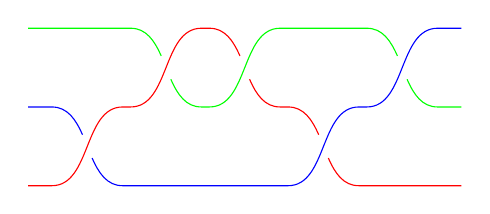
\begin{tikzpicture}
\braid[
  number of strands=3,rotate=90,style strands={1}{red},style strands={2}{blue},style strands={3}{green}
 ](braid at (2,0) a_1 a_2 a_2 a_1 a_2 ;
 %\fill[purple] (braid) circle (4pt);
\end{tikzpicture} 
\caption{A braid with three strands.}
\label{fig:BRAID}
\end{center}
\end{figure}

A braid \cite{Kaufman_et_al:2006} is an embedding of a collection of strands that have their ends in two rows of points that are set one above the other with respect to a choice of vertical. The strands are not individually knotted and they are disjoint from one another. Figure~\ref{fig:BRAID} shows an example of a braid with three strands. 


A braid operation can be represented by a matrix that acts on the qubit space. These matrices are referred to as generators, and the quantum gate that a braid represents is the product of the generators that encode the individual braid operations. The braid group $B_n$ is defined by a set of generators $\sigma_1,\dots,\sigma_n$ that satisfy the following relationships:
 \begin{align}
  \sigma_i \sigma_k &= \sigma_k \sigma_i \; \; \text{if} |i-k| \geq 2 \\
    \sigma_i \sigma_{i+1} \sigma_i &=  \sigma_{i+1} \sigma_i \sigma_{i+1} 
 \end{align}

We work with braids of three strands that can be represented by two generators. Let $\sigma_1$ and $\sigma_2$ represent two possible generators.  $\sigma_1^{-1}$   and $\sigma_2^{-1}$ respectively represent their inverses. 


\begin{equation}
\sigma_1 =  \left( \begin{array}{cc}
e^{\frac{-i7\pi}{10}}   & 0 \\
0 & -e^{\frac{-i3\pi}{10}}   \end{array} \right) 
\hspace{1.0cm} 
\sigma_2 =  \left( \begin{array}{cc}
-\tau e^{\frac{-i \pi}{10}}   & -i \sqrt{\tau} \\
-i \sqrt{\tau} & -\tau e^{\frac{-i\pi}{10}}   
\end{array} \right) \label{eq:SIG2}
\end{equation}
where $\tau = \frac{\sqrt{5} -1}{2}$. 

Given a braid $B$, $len()$ is a function that  returns the braid's length $l$ (e.g. $B=\sigma_1 \sigma_1 \sigma_2 \sigma_1^{-1}$, $l=len(B)=4$). Since the product of a matrix by its inverse  reduces to the identity matrix, some braids can be simplified reducing their length. Therefore, we also define function $elen()$, that has a braid as its argument and returns the braid's \emph{effective length} which is the length of braid after all possible simplifications have been conducted.

\begin{align}
  \sigma_1 \sigma_1 \sigma_1 \sigma_1 \sigma_1^{-1} =&   \sigma_1 \sigma_1 \sigma_1 \label{eq:EL1} \\
  \sigma_2^{-1} \sigma_1 \sigma_1 \sigma_1^{-1} \sigma_1^{-1}  \sigma_2 \sigma_1^{-1} =& \sigma_1^{-1} \label{eq:EL2} 
\end{align}

 In the braids shown in examples \eqref{eq:EL1} and  \eqref{eq:EL2}, the effective length values are $3$ and $1$, respectively. 

Let $T$ represent the target matrix (gate to be emulated), the braid error is calculated with the following metric  \cite{Mcdonald_and_Katzgraber:2013}:
\begin{equation}
 \epsilon = |B-T| \label{eq:ERROR}
\end{equation}
where the matrix norm used is
\begin{equation}
 |M| = \sqrt{\sum_{ij}M_{ij}^2}.
\end{equation}

The problem of finding braiding operations that approximate gates is then reduced to finding a product chain of the reduced generators and their inverses that approximates the matrix representing the quantum gate. Two elements that describe the quality of a braid are its error $\epsilon$ and its length $l$. 




 In this paper we address the problem of finding a product of generator matrices that approximates a given target $T$. The search for the product of generators is approached as a combinatorial problem defined in the space of all possible braids of size $n$.  Although the methodology we propose can be extended to other braids, we focus on anyon braids since they are one of the best known in TQC \cite{Mcdonald_and_Katzgraber:2013,Xu_and_Xin:2008}.


\section{Problem formulation} \label{sec:PROBFORM}

%\subsection{Problem representation}


Let ${\bf{X}}=(X_1,\ldots ,X_n)$ denote a vector of discrete random variables. We use ${\bf{x}}=(x_1,\ldots ,x_n)$ to denote an assignment to the variables. $I$ denotes a set of indices in $\{1, \ldots, n\}$, and $X_I$ (respectively $x_I$) a subset of the variables of ${\bf{X}}$ (respectively ${\bf{x}}$) determined by the indices in $I$.

 In our representation for the quasiparticle braids problem,  ${\bf{X}}=(X_1,\ldots ,X_n)$ represents a braid of length $n$, where  
$X_i$ takes values in $\{0,1, \dots, 2g-1\}$ and $g$ is the number of generators. Given an order for the generators $\sigma_1, \sigma_2, \dots, \sigma_g$,  $X_i=j, j<g$ means that the matrix in position $i$ is $\sigma_{j+1}$. If $X_i =j, j \geq g$, then the matrix in position $i$ is $\sigma^{-1}_{(j-g)+1}$.  For example, for generators shown in Equation~\eqref{eq:SIG2}, and  $B=\sigma_1 \sigma_1 \sigma_2 \sigma_2^{-1} \sigma_1^{-1}$, the corresponding braid representation is  ${\bf{x}}=(0,0,1,3,2)$. Notice that this is a fixed length representation. 


%\subsection{Fitness function}

We are interested in the solution of an optimization problem formulated as   ${\bf{x}}^* = arg max_{{\bf{x}}} f({\bf{x}})$,  where $f : S \rightarrow R$ is called the objective or fitness function. The optimum   ${\bf{x}}^*$ is not necessarily unique. To evaluate the fitness function associated to a solution ${\bf{x}}$, firstly the product of braid matrices $B$ is computed according to ${\bf{x}}$ and then the error $\epsilon$ is calculated from $B$ as in Equation~\eqref{eq:ERROR}. 

The fitness function  \cite{Mcdonald_and_Katzgraber:2013} is defined as:
\begin{equation}
 f({\bf{x}}) = \frac{1-\lambda}{1+\epsilon} + \frac{\lambda}{l} \label{eq:FITNESS}
\end{equation}
where $l$ is the braid's length, and $\lambda$ serves to balance the two conflicting goals, i.e., having short braids or low approximation error. When $\lambda=0$, braids are optimized only for the error and the function reaches its maximum value when this error is minimized. 

 We define functions $\hat{f}({\bf{x}})$ and  $\bar{f}({\bf{x}})$ as two variations of function~\eqref{eq:FITNESS}. Function  $\hat{f}({\bf{x}})$ is identical to $f({\bf{x}})$, except that the effective length $\hat{l}=elen(B)$ is used instead of the braid's length. Function $\bar{f}({\bf{x}})$ outputs the maximum value of the function for any of the braids contained in $B$ that start from the first position, i.e. 

\begin{equation}
     \bar{f}({\bf{x}}) =  max_{{\bf{y}}, {\bf{y}} \in \{(x_1),(x_1,x_2),\dots,(x_1, \dots,x_i), \dots, (x_1,\dots,x_n)\}} f({\bf{y}})
\end{equation}


\section{Estimation of distribution algorithms} \label{sec:EDAs}


 EDAs assume that some  statistical regularities in the best solutions exist and that these regularities can be used to bias the search to the promising areas of the search space. Therefore, it is important to determine whether such assumption holds for the braid problem.  In \cite{Santana_et_al::2014a}, we have investigated whether possible regularities of the search space for the braid problem can be detected from the statistical analysis of the Boltzmann distribution \cite{Muehlenbein_and_Mahnig:2002a} defined on the braid function.  Similar analysis has been successfully applied to investigate the dependencies that arise in the configurations of simplified protein models \cite{Santana_et_al:2008a} and conductance-based neuron models \cite{Santana_et_al:2012h}.

 
 Our analysis showed that there are at least two types of regularities of the braid problem that are translated into statistical features. Firstly, there are different frequencies associated to the generators in the space of the best solutions. Secondly, there are strong dependencies between the variables, particularly those that are adjacent in the braid representation. This evidence can be useful to explain the results of different variants of EDAs for this problem. In this section we describe the main characteristics of the EDAs used to solve the braid problem. 


\subsection{EDA approach}



 The pseudocode of a general EDA is shown in Algorithm~\ref{alg:EDA}. The organization of the algorithm and the evaluation and selection steps are similar to a genetic algorithm. The main differences are in step $5$ the algorithm, where a probabilistic model is learned from the data, and in step $6$, where the model is used to sample the new solutions of the population. We use as a termination criterion a maximum number of generations. Truncation selection was used, in which the best $5\%$ of the population is selected according to the fitness values.  Finally, in order to form the new population, the new sampled solutions are combined with the set of best solutions (elitist solutions) selected from the current generation and the wort solutions are removed. 

 

  
\begin{BAlgo}{Estimation of distribution algorithm}
 \label{alg:EDA}
 \item Set $t\Leftarrow 0$. Generate $N$ solutions randomly.
 \item \Do
 \item \T {Evaluate the solutions using the fitness function.}
 \item \T {Select a population $D_t^S$ of $K \leq N$ solutions according to a selection
method.}
 \item \T {Calculate a probabilistic model of $D_t^S$.}
 \item \T {Generate $N$ new solutions sampling from the distribution represented
in the model and combine with current population.}
 \item \T {$t \Leftarrow t+1$}
 \item  \Until{Termination criteria are met.}
\end{BAlgo}





\subsection{Probabilistic models}

 One relevant question for solving combinatorial problems using EDAs is which is the type and amount of interactions between the variables of the problem that should be modeled in order to find the optimal solutions. Different probabilistic models are able to represent different number of interactions but usually, as this capacity increases, the computational cost of the algorithm also grows. We investigate three EDAs that differ in the probabilistic models they use and that have been previously applied to a variety of combinatorial problems and~\cite{Armananzas_et_al:2008,Baluja_and_Davies:1997r,DeBonet_et_al:1996r,Echegoyen_et_al:2012a,Santana_et_al:2008a}. It follows a description of the models:


 We work  with positive distributions denoted by $p$. $p(x_I)$ denotes  the  marginal probability for ${\bf{X}}_I={\bf{x}}_I$.   $p(x_i \mid x_j)$ denotes the conditional probability distribution of $X_i=x_i$ given $X_j=x_j$. Three types of probabilistic graphical models are defined: 1) Univariate model. 2) $1$-order Markov model. 3) Tree model. 


In the univariate model variables are considered to be independent, and the probability of a solution is the product of the univariate probabilities for all variables:

\begin{equation}
 p_{u}({\bf{x}}) =   \prod_{i=1}^{n}  p(x_{i}) \label{eq:UNIV}
\end{equation}

We call the EDA that uses the univariate probabilistic model as univariate marginal distribution algorithm (UMDA) \cite{Muhlenbein_and_Paas:1996r}. 

In the $1$-order Markov model, the configuration of variable $X_i$ depends on the configuration of the previous variable in the solution:

\begin{equation}
 p_{MK}({\bf{x}}) =  p(x_{1})  \prod_{i=2}^{n}  p(x_{i} \mid  {x_{i-1}}) \label{eq:MKFACT}
\end{equation}

The EDA that uses the  $1$-order Markov model is called in this paper Mk-EDA. 

  A probability distribution $p_{\mathcal{T}}({\bf x})$ that is conformal with a tree is defined as:
\begin{equation}
  p_{\mathcal{T}} ({\bf{x}}) =\prod_{i=1}^{n} p(x_i|pa(x_i)),
\end{equation}
 where $Pa(X_i)$  is the parent of $X_i$ in the tree, and $p(x_i|pa(x_i))=p(x_i)$ when $pa(X_i)=\emptyset$, i.e. $X_i$ is a root of the tree. We allow the existence of more than one root in the PGM (i.e. forests) although for convenience of notation we refer to the model as tree. 
 
The EDA that uses the  tree model is called in this paper Tree-EDA.

 Univariate approximations are expected to work well for functions that can be additively decomposed into  functions of order one (e.g. $g({\bf{x}})= \sum_i x_i$). However, other non additively decomposable functions can be easily solved with EDAs that use univariate models (e.g. $g({\bf{x}})=   \prod_i x_i + \sum_i x_i $) \cite{Muhlenbein_et_al:1999}. Therefore, it makes sense to test the univariate approximation for the braid problem.  


The $1$-order Markov model  captures only dependencies between adjacent variables. Learning of the model implies learning the conditional pairwise dependence relationships between the adjacent variables. During the sampling process, first variable $X_1$ is sampled, and every other variable $X_i$ is sampled conditioned on $X_{i-1}$.  


The tree model can represent a maximum of $n-1$ bivariate dependencies and is the only model among the three for which the structure of the dependencies between the variables has to be learned from the data. The  construction of the tree structure from data implies the detection of the most important bivariate interactions between the variables. Initially, the univariate and bivariate probabilities are respectively calculated for every variable and pair of variables.  From these marginal probabilities, the mutual information between each pair of variables is computed. To construct the tree structure, the Chow-Liu algorithm \cite{Chow_and_Liu:1968} is used.  It finds the maximum  weight spanning tree  from the matrix of mutual information between pairs of variables. Probabilistic logic sampling (PLS) \cite{Henrion:1988} is applied to sample new solutions from the tree.


The computational cost of EDAs is mainly associated to the methods needed to learn and sample the models. The most complex EDA used in this paper is Tree-EDA which has a computational cost $O(n^2)$. Examples of EDAs that use univariate, $1$-order Markov, and tree models  are respectively presented in \cite{Muhlenbein_and_Paas:1996r}, \cite{DeBonet_et_al:1996r} and~\cite{Baluja_and_Davies:1997r,Santana_et_al:2008a} and details on the methods used to learn and sample the models can be obtained from these references. 


 \subsection{Enhancements to the EDAs} \label{sec:ENH}

   We consider three enhancements to EDAs: 1) Use of a local optimizer. 2) Partial sampling. 3) Recoding. 
 
   As is the case of other EAs, EDAs can be enhanced by the incorporation of local optimizers \cite{Pelikan_and_Goldberg:2003,Santana_et_al:2008f}. We use a greedy optimization algorithm that is applied during the evaluation of the population by the EDA.  The algorithm starts from the solution generated by the EDA. In each iteration, the local optimizer evaluates all the $3n$ solutions that are different to the current solution in only one variable (the neighbor solutions). The next selected solution is the neighbor that improves  the fitness of the current solution the most. The algorithm stops when none of the neighbors improves the fitness of the current solution. 
 
  During the sampling step of an EDA, all variables are assigned their values according to the probabilistic model and the sampling method. For the EDA that uses the univariate model, variables are independently sampled. For 1-order Markov and tree, PLS \cite{Henrion:1988} is used. In both methods, all variables are assigned the new values. However, for some problems with higher-order interactions using a base-template solution can be better than generating each new solution from scratch. 

 In partial sampling \cite{Pereira_et_al:2000,Tsutsui_et_al:2003}, a solution of the population is selected and only a subset of its variables are sampled according to the model. We use two variants of partial sampling I) Partial sampling where the number of variables to be modified is randomly selected between $1$ and $n$. II)  Partial sampling, where  the number of variables to be modified is randomly selected between $1$ and $\frac{n}{2}$.

  Recoding consists in modifying the representation of the solution after  the fitness evaluation. For functions $\hat{f}$ and $\bar{f}$ it is possible to recode the solution by eliminating redundant generators (e.g.,  pairs $\sigma_i \sigma_i^{-1}$). The rationale of using recoding is that meaningful variables will be located closer to the beginning of the braid. Since solutions have a fixed length, the last variables will be kept unused, i.e. garbage information. Therefore, we devised two ways to fill these gaps: I) Leaving the unused variables as they were in the original solution. II) Replacing the unused variables by a reverse copy of the variables used in the evaluation. The second variant intends to replicate information that has proved to be ``informative'' about the problem. Equations~\eqref{eq:EX3} and~\eqref{eq:EX4} show examples of recoding type I and II, respectively. In this hypothetical examples, the underlined variables are those that provided the best fitness after simplifying the braid and evaluating function $\bar{f}$.  

\begin{align}
   (\underline{0,3},1,3,\underline{3,3,2},1,2,2) =&  (\underline{0,3,3,3,2},3,2,1,2,2) \label{eq:EX3} \\
(\underline{0,3},1,3,\underline{3,3,2},1,2,2) =&  (\underline{0,3,3,3,2},2,3,3,3,0) \label{eq:EX4} 
\end{align}
 
% The Boltzmann distribution has played an important role in the theoretical analysis of EDAs and other authors have analyzed the relationship between the function structure and the dependencies in the distribution \cite{Muehlenbein_and_Mahnig:2000}. Other problems from physics have been previously treated with EDAs. In particular, spin glass models with different types of interactions and topologies have been addressed \cite{Pelikan_and_Katzgraber:2009}. Two important differences between the braid problem and the spin glass models that makes it particularly challenging is that its fitness function is multiplicative and that the representation is non binary. In fact, the  cardinality of the variables can increase with the number of generators.  We did not find any previous reference on the use of  probabilistic graphical models or machine learning methods to compute quasiparticle braids.

     

\section{Related work} \label{sec:RELWORK}


 In addition to genetic algorithms  \cite{Mcdonald_and_Katzgraber:2013}, other approaches have been applied to the quantum gate approximation problem.

 \subsection{Solovay-Kitaev algorithm}
 
   The Solovay-Kitaev algorithm \cite{Kitaev:2003,Dawson_et_al:2005} is a constructive procedure that guarantees to obtain a braid approximation of a single-qubit gate with an arbitrary error $\epsilon$. The algorithms uses as input a library set of gates $\{L_1,L_2,\dots,L_k\}$ and recursively constructs a combination of these gates that minimizes the error until achieving the desired error.
     The Solovay-Kitaev theorem states \cite{Trung_et_al:2012} that, for a given gate $G$, error $\epsilon$, and library set $\{L_i\}$, there always exists a sequence of library gates $(\prod_{j=1}^{l}A_j | A_j \in  {L_i}{L_i^{-1}})$ such that \cite{Dawson_et_al:2005}:

\begin{equation}
 \| G- \prod_lA_l\| \leq \epsilon
\end{equation}
Furthermore, it is possible to set the dependence between the length of the sequence ($l$) and $\epsilon$ as $l=O[log^{c}(1/\epsilon)]$, where the Solovay-Kitaev standard algorithm gives a scaling of sequence size according to $c=3.97$. 


 One drawback of the standard Solovay-Kitaev algorithm is that in each iteration the braid length increases by a factor of $5$. As a result, there may be shorter braids that achieve the same precision of the braid produced by the algorithm. Another factor that influences the behavior of the standard Solovay-Kitaev algorithm is that, at its first layer, it conducts an exhaustive search over the space of braids up to length $l_0$. Obviously, such sort of exhaustive search is only feasible for small values of $l_0$. Recently, improved variants of the standard Solovay-Kitaev algorithm have been proposed \cite{Trung_et_al:2012}.


\subsection{Geometrical approaches} 

 Other approaches \cite{Burrello_et_al:2010,Burrello_et_al:2011,Mosseri:2008} try to construct an initial braid approximation of the target gate and then refine this approximation. The way refinement is conducted is similar to the idea of hashing as applied for data indexing in computer science. The key question is how to define the hashing table that allows to efficiently improve the braid approximations. 

 We present in some more detail the quantum hashing method since one of the problems addressed in the section of experiments is inspired in this work.
 
 \subsubsection{Quantum hashing with the icosahedral group} \label{sec:ICOSA}

Braid generators are unitary matrices, i.e. square matrices $U$ that satisfy that $U^H=U^{-1}$, where $U^H$ denotes the conjugate transpose and $U^{-1}$ is the matrix inverse. The special unitary group $SU(2)$ is the group of all $2 \times 2$ unitary matrices with determinant $1$. The $3d$ rotation group $SO(3)$ is the group of all rotations about the origin of three-dimensional Euclidean space $\mathcal{R}^3$ under the operation of composition. The quantum hashing procedure presented in  \cite{Burrello_et_al:2010,Burrello_et_al:2011} uses the homomorphism between $SU(2)$ and $SO(3)$ to associate a $2 \times 2$ unitary matrix to each element of the icosahedral rotation group
$\mathcal{I}=\{g_1,\dots,g_{60}\}.$

 The icosahedral group comprises the $60$ rotations around the axes of symmetry of the icosahedron. Each of these rotations is initially approximated by a braid of fixed length $L$ that is searched using brute-force. The resulting approximation of the group $\mathcal{I}$ is then defined as $\tilde{\mathcal{I}}=\{\tilde{g}_1,\dots,\tilde{g}_{60}\}$. The elements of $\tilde{\mathcal{I}}$  are then used to find a combination of $m$ elements that produces a rough braid representation of any target quantum gate $T$.  Finally, the rough approximation of $T$ is refined by conducting another search in another set of braid approximations found by applying brute-force in the search space of larger braids. In our experiments we use EDAs to find braid approximations of all the elements of $\mathcal{I}$. 


\subsection{Brute-force methods}


 Brute-force has been extensively applied to search for braids of manageable size. As mentioned before, the  Solovay-Kitaev algorithm and the quantum hashing method apply a preliminary exhaustive search to find the initial qubit approximations. For instance, in  \cite{Bonesteel_et_al:2005} brute-force is used to optimize braids of length up to $46$. The quantum hashing method presented in  \cite{Burrello_et_al:2010} applies brute-force to find braids of $L=24$, and in  \cite{Burrello_et_al:2011} the $60$ elements of the icosahedral group are approximated with braids up to length $L=68$. The high computational cost of such an exhaustive search is justified because once the braids are found they may be reused many times to approximate other targets. However, it is clear that brute-force is not feasible for higher $L$. 

It is remarkable that, with the exception of GAs, other combinatorial optimization algorithms have not been applied as part of the Solovay-Kitaev algorithm and the quantum hashing method to create more accurate initial braids of medium and large size. Combinatorial optimization methods allow  the user to  tune the balance between the error and the length of the braid  and provide different solutions to the problem. 
  
%  Other methods such as the Solovay-Kitaev algorithm \cite{Dawson_et_al:2005,Hormozi_et_al:2007,Nielsen_and_Chuang:2010} provide bounds on the accuracy and length of the braids. 


  


  \subsection{Application of EDAs to problems from Physics} 
 
  Other problems from physics have been previously treated with EDAs. In particular, spin glass models with different types of interactions and topologies have been addressed \cite{Pelikan_and_Goldberg:2003r,Pelikan_and_Katzgraber:2009,Shakya_et_al:2011,Shakya_and_Santana:2012}. Two important differences between the braid problem and the spin glass models that makes it particularly challenging is that its fitness function is multiplicative and that the representation is non binary. In fact the  cardinality of the variables can increase with the number of generators.  



\section{Experiments} \label{sec:EXPE}

  The main objective of our experiments is to evaluate the capacity of the EDAs to find optimal solutions to the quantum gate approximation problem. A second objective is to evaluate different variants of the algorithm and compare their results to other methods. 


\subsection{Experimental settings}

Each EDA is characterized by $5$ parameters:

\begin{itemize}
\item   Use of local optimizer. 0: Only EDA is applied, 1: EDA is combined with greedy search as described in Section \ref{sec:ENH}. 
\item  Type of function and representation. 0: Function $f$,  1: Function $\bar{f}$ without recoding, 2: Function $\bar{f}$ with recoding I, 3: Function $\bar{f}$ with recoding II.
 \item  $\lambda$ value.  0:0.0, 1:0.01, 2:0.05, 3:0.1. 
 \item  Sampling method. 0: Normal, 1: Partial sampling I,  2: Partial sampling II. 
 \item  Type of probabilistic model. 0: Univariate, 1: 1-order Markov, 2: Tree.
\end{itemize}



The experimental settings were selected to investigate different aspects that influence the behavior of the algorithm. For the first problem addressed, we run experiments for $n \in \{50,100,150,200,250\}$ in order to evaluate the scalability of the algorithms. Increasing $n$ may lead to obtain braids with a smaller error. 


The total number of variants of the algorithm was $2 \times 4 \times 4 \times 3 \times 3 = 288$. All the algorithms use truncation selection, in which the best $5\%$ of the population is selected. EDAs that do not incorporate the greedy local search use a population size $N=10000$. For these EDAs, the number of generations  was dependent on $n$ as $N_g = 15n$. Due to the large number of evaluations spent by the greedy search method, the population size for all hybrid EDAs was $N=100n$ and the number of generations was fixed to  $N_g = 100$. For each EDA variant, $100$ experiments were run.  

\subsection{Problem benchmark}

 Target gates define different instances of the braid problem. Additionally, the maximum posible length of the braid solutions behave as contraints for the precision of the best approximation. In our experiments we use different target gates and  different braid lengths. 

 The first target ($T_1$) was the one used in \cite{Mcdonald_and_Katzgraber:2013} to evaluate the performance of the introduced GA. 

\begin{equation}
  T_1 = \left( \begin{array}{cc}
  0   & i  \\
  i & 0   
  \end{array} \right)
\end{equation}

The results obtained on target $T_1$ allowed us to identify the best EDA variant which was then applied to another set of $60$ target gates, those unitary matrices that belong to the icosahedral group $\mathcal{I}$ explained in Section~\ref{sec:ICOSA}. The definition and implementation of the group elements were obtained from the original code\footnote{\url{https://sites.google.com/site/braidanyons/download}} available from the authors of \cite{Burrello_et_al:2010,Burrello_et_al:2011}. 


\subsection{Results for target $T_1$}


%\subsubsection{Best solutions found by EDAs}

Figure~\ref{fig:RHCSTEPS}a)  and Table~\ref{tab:BESTSOL} respectively show  the parameters that characterize the best braids found by the EDAs for each value of $n$,  and the braids. In Figure~\ref{fig:RHCSTEPS}a), we also show an estimate of the length  of the braids ($O[log_{10}^{3.97}(1/\epsilon)]$) that would compute the Solovay-Kitaev algorithm  \cite{Dawson_et_al:2005} to obtain the same error $\epsilon$ of our best solutions. The lengths of our solutions clearly outperform these estimates. Figure~\ref{fig:RHCSTEPS}b) shows the length of all the best solutions achieved for each value of $n$. It can be observed in Figure~\ref{fig:RHCSTEPS}  that EDAs are able to find several braids with different lengths for $n=150$ and $n=200$. 


\subsubsection{Behavior of the EDA variants}


\begin{figure}[htbp]
%\scriptsize
\begin{center}
 \begin{pspicture}(0,0)(10.0,3)
\rput[l](-1,1){
\begin{array}{|c|r|c|c|c|} \hline 
n & l & \epsilon & log_{10}(\epsilon) &  log_{10}^{3.97}(\frac{1}{\epsilon})  \\ \hline
50 & 44 & 4.8435 \times 10^{-4} & -3.3148 & 116.47\\  \hline
100 &70  &8.3527 \times 10^{-6} & -5.0782 & 633.37 \\ \hline
150 &64 & 8.3527 \times 10^{-6} & -5.0782 & 633.37 \\ \hline
200 &62 & 8.3527 \times 10^{-6} & -5.0782&  633.37 \\  \hline
250 &124 & 3.5038 \times 10^{-6} & -5.4555 & 841.82\\ \hline
\end{array}}
\rput[l](5.5,1){\includegraphics[width=5.5cm]{newBestSolsDist.eps}}
\end{pspicture}
\begin{pspicture}(0,-0.25)(12,0)
    \rput(3.0,-0.5){a)} \rput(9.5,-1.5){b)}  %\rput(12.0,-0.125){c)}
\end{pspicture}
\end{center}
\vspace{0.7cm}
  \caption{Target $T_1$: a) Parameters of the best braids found by the EDAs for each value of $n$. b) Length of the best solutions found for each value of $n$.}
  \label{fig:RHCSTEPS}   
\end{figure}  
 
 We further investigate the behavior of the different EDA variants. Figure~\ref{fig:VIO} shows the violin plots \cite{Hintze_and_Nelson:1998} with the distribution of the best values found in all the executions for: a) All EDA variants without local optimizer ($14400$ runs) and b) EDAs with local optimizer, recoding type II, and that use partial sampling type II ($300$ runs). Each violin plot shows a  histogram  smoothened using a kernel density with Normal kernel.  The mean and median are shown as red crosses and  green squares, respectively.



\begin{table*} 
\scriptsize
\begin{center}
 {$ \begin{array}{|c|l|} \hline 
n &  \multicolumn{1}{c|}{\text{braid}}  \\ \hline  \hline
50 &  \sigma_1^{-1}\sigma_2^{3}\sigma_1^{-2}\sigma_2\sigma_1^{-1}\sigma_2\sigma_1^{-2}\sigma_2^{3}\sigma_1^{-1}\sigma_2\sigma_1^{-1}\sigma_2\sigma_1^{-2}\sigma_2\sigma_1^{-2}\sigma_2\sigma_1^{-1}\sigma_2^{3}\sigma_1^{-1}\sigma_2^{2}\sigma_1^{-1}\sigma_2\sigma_1^{-1}\sigma_2\sigma_1^{-2}\sigma_2^{2}\\ 
& \sigma_1^{-3}\sigma_2^{2}  \\  \hline

100 & \sigma_1\sigma_2^{-2}\sigma_1^{4}\sigma_2^{-1}\sigma_1\sigma_2^{-4}\sigma_1\sigma_2^{-1}\sigma_1^{3}\sigma_2^{-1}\sigma_1^{2}\sigma_2^{-2}\sigma_1^{4}\sigma_2^{-1}\sigma_1\sigma_2^{-4}\sigma_1\sigma_2^{-1}\sigma_1^{6}\sigma_2^{2}\sigma_1\sigma_2\sigma_1\sigma_2^{2}\sigma_1^{3}\sigma_2^{5}\sigma_1^{-1}\sigma_2 \\
& \sigma_1^{-3}\sigma_2\sigma_1^{3}\sigma_2^{5} \\ \hline

150 & \sigma_2\sigma_1^{-1}\sigma_2\sigma_1^{-1}\sigma_2^{-1}\sigma_1^{2}\sigma_2^{-1}\sigma_1\sigma_2^{-4}\sigma_1^{2}\sigma_2^{-2}\sigma_1^{-1}\sigma_2^{-1}\sigma_1^{-2}\sigma_2^{-4}\sigma_1^{2}\sigma_2^{-4}\sigma_1\sigma_2^{-1}\sigma_1^{2}\sigma_2^{-1}\sigma_1^{-1}\sigma_2\sigma_1^{-3}\\ 
& \sigma_2^{-1}\sigma_1\sigma_2^{-1}\sigma_1^{3}\sigma_2^{-1}\sigma_1\sigma_2^{-4}\sigma_1^{2}\sigma_2^{-4}\sigma_1^{2}\sigma_2^{-3}\\ \hline

200 & \sigma_2^{-2}\sigma_1^{4}\sigma_2^{-1}\sigma_1\sigma_2^{-4}\sigma_1\sigma_2^{-1}\sigma_1^{2}\sigma_2^{-1}\sigma_1^{3}\sigma_2^{-1}\sigma_1\sigma_2^{-4}\sigma_1\sigma_2^{-1}\sigma_1^{4}\sigma_2^{-1}\sigma_1\sigma_2^{-2}\sigma_1^{2}\sigma_2^{2}\sigma_1\sigma_2^{-1}\sigma_1\sigma_2^{-1}\sigma_1^{-5}\\
&\sigma_2\sigma_1^{-1}\sigma_2^{-6}\sigma_1^{-2}\sigma_2^{3} \\  \hline

 250 & \sigma_1\sigma_2\sigma_1^{-1}\sigma_2\sigma_1^{-1}\sigma_2^{-1}\sigma_1\sigma_2^{-1}\sigma_1^{-3}\sigma_2^{4}\sigma_1^{-2}\sigma_2^{4}\sigma_1^{-1}\sigma_2\sigma_1^{2}\sigma_2\sigma_1^{-1}\sigma_2^{4}\sigma_1^{-2}\sigma_2^{4}\sigma_1^{-3}\sigma_2^{-1}\sigma_1\sigma_2^{-1}\sigma_1^{-1}\sigma_2^{2}\\

&\sigma_1\sigma_2^{-1}\sigma_1^{2}\sigma_2^{-1}\sigma_1\sigma_2^{-4} \sigma_1^{2}\sigma_2^{-4}\sigma_1\sigma_2^{-1}\sigma_1^{4}  \sigma_2^{-1}\sigma_1^{-1}\sigma_2^{-1}\sigma_1^{-4}\sigma_2^{-1}\sigma_1^{-1}\sigma_2^{-1}\sigma_1^{4}\sigma_2^{-1}\sigma_1\sigma_2^{-4}\sigma_1^{2}\sigma_2^{-4}\\
&\sigma_1\sigma_2^{-2}\sigma_1^{-1}\sigma_2^{5}\sigma_1^{-1}\sigma_2\sigma_1^{-4}\sigma_2^{2}\sigma_1^{-4}\sigma_2^{2}\sigma_1^{-4}\sigma_2^{2}\sigma_1^{-1} \\ \hline
\end{array}$}
\end{center}
\caption{Best braids found by the EDAs for each value of $n$.}
\label{tab:BESTSOL}
\end{table*}

\begin{figure*}[htbp]
  \begin{center}
    %\includegraphics[width=4.0cm]{newViolinOnlyEDA.eps}
    \includegraphics[width=5.8cm]{newViolinEDAGreedy.eps}
    \includegraphics[width=5.8cm]{newViolinF7Dist.eps}
\begin{pspicture}(0,-0.25)(12,0)
    \rput(3.5,-0.125){a)} \rput(9.0,-0.125){b)}
\end{pspicture}
     \caption{Results for target $T_1$ a) All EDAs variants with local optimizer  ($14400$ runs), b) EDAs with local optimizer, recoding type II, and that use partial sampling type II ($300$ runs).}
    \label{fig:VIO}
    \end{center}
\end{figure*}

 In Figure~\ref{fig:VIO}, the modes  of the Normal distribution indicate the existence of a local optimum of the error with a very wide basin of attraction. This local optimum has value $log_{10}f(\epsilon) = -2.50785$ and the majority of the EDA runs can be trapped in this value. Figure~\ref{fig:VIO}b) reveals how a particular combination of the EDA's parameters can improve the results of the search.  This is shown in detail in Table~\ref{tab:F5RES} that comprises  all EDA variants that reached one of the best solutions in at least one of the $100$ runs. 


\begin{table}[htb]
\scriptsize
\begin{center}
 {$ \begin{array}{|r|r|r|r|r||r|r|r|r|r|r|||r|r|r|r|r||r|r|r|r|r|r|} \hline 
  L & tf& t \lambda & ts & pm &50 & 100 &150 & 200 &250 & tot & L & tf& t \lambda & ts & pm &50 & 100 &150 & 200 &250 & tot \\ \hline\hline 
  0&3& 1& 0& 0& 0& 0& 1& 1& 0& 2 & 1&2& 2& 1& 2& 0& 0& 1& 0& 0& 1\\  
  0&3& 1& 1& 0& 1& 0& 1& 4& 0& 6 &  1&3& 0& 1& 2& 0& 0& 1& 0& 0& 1\\ 
  0&3& 1& 1& 1& 0& 0& 1& 2& 0& 3 &  1&3& 1& 1& 0& 0& 0& 0& 2& 0& 2\\ 
  0&3& 1& 1& 2& 0& 0& 1& 0& 0& 1 &  1&3& 1& 1& 2& 0& 0& 0& 1& 0& 1\\ 
  0&3& 1& 2& 0& 0& 0& 0& 2& 0& 2 &  1&3& 1& 2& 0& 0& 0& 9& 12& 0& 21\\
  0&3& 1& 2& 1& 0& 0& 0& 2& 0& 2 &  1&3& 1& 2& 1& 0& 2& 14& 21& 0& 37\\ 
  0&3& 1& 2& 2& 0& 0& 0& 3& 1& 4 &  1&3& 1& 2& 2& 0& 1& 18& 19& 0& 38\\        
  0&3& 2& 0& 0& 0& 0& 0& 1& 0& 1 &   1&3& 2& 1& 0& 0& 0& 0& 4& 0& 4\\  
  0&3& 2& 1& 0& 0& 0& 4& 3& 0& 7 &   1&3& 2& 1& 1& 0& 0& 1& 1& 0& 2\\ 
  0&3& 2& 1& 1& 0& 0& 0& 1& 0& 1 &   1&3& 2& 1& 2& 0& 0& 1& 0& 0& 1\\ 
  0&3& 2& 1& 2& 0& 0& 1& 1& 0& 2 &   1&3& 2& 2& 0& 0& 0& 4& 20& 0& 24\\ 
  0&3& 2& 2& 0& 0& 1& 0& 1& 0& 2 &   1&3& 2& 2& 1& 0& 0& 2& 9& 0& 11\\ 
  0&3& 2& 2& 1& 0& 1& 1& 1& 0& 3 &   1&3& 2& 2& 2& 0& 0& 4& 11& 1& 16 \\
  0&3& 2& 2& 2& 0& 0& 2& 3& 0& 5 &    & &  &  &  &  &  &  &   &  &  \\\hline     
\end{array}$}
\caption{Results target $T_1$: EDA variants that reached one of the best solutions in at least one in the $100$ experiments. $L$: Local optimizer, tf: Type of function and representation, $t\lambda$: type of $\lambda$ value, $ts$: type of sampling, $pm$: probabilistic model.}
\label{tab:F5RES}
\end{center}
\end{table}


 There are a number of commonalities between the best EDA variants. Except in one case, all EDAs use recoding of type II. Similarly, except in one case, in all the variants $\lambda \in \{ 0.01, 0.05\}$. Except in two cases, the sampling method selected was partial sampling. The application of the local optimizer notably improved the results for $n \in \{150, 200\}$ but in terms of the best solution found it did not have an important influence for the other values of $n$. 

 As a summary, we recommend to use an EDA that adds the greedy search, and uses recoding of type II, partial sampling and the 1-order Markov model since it is less complex than the tree and results achieved using the two models are similar.
  
\subsubsection{Improvement over other search methods}

  We compare our best EDA variant with the results achieved using a random search, the greedy local optimizer, and the GA introduced in \cite{Mcdonald_and_Katzgraber:2013}. For the random search, we randomly generated $10000$ solutions and selected the best solution according to function $\bar{f}, \lambda = 0.01$. The same experiment was repeated $100$ times to select the $100$ ``best'' solutions for $n \in \{50,100,150,200,250\}$.



\begin{figure}[htbp]
  \begin{center}
 \includegraphics[width=5.8cm]{newBoxPlotn50.eps}
 \includegraphics[width=5.8cm]{newBoxPlotAllns.eps}
\begin{pspicture}(0,-0.25)(12,0)
    \rput(3.5,-0.125){a)} \rput(9.0,-0.125){b)}
\end{pspicture}
  \caption{a) Comparison between the Best EDA variant, the random search, the greedy local search and the GA for $n=50$. b) Comparison between the Best EDA variant and the greedy local search  $n \in \{100,150,200,250\}$.}
    \label{fig:BPn50}   
 \end{center}
\end{figure}  


 A similar procedure was followed for the greedy local search. The local optimizer was applied to each of the $10000$ solutions until no improvement was possible. For the GA, we used the results of the $100$ GA runs analyzed in \cite{Mcdonald_and_Katzgraber:2013}. Since these results were obtained using solutions of different length, and with a different number of evaluations, care must be taken to interpret the differences. We only compare the GA results with the other algorithms for $n=50$. Similarly, the results of the random search were very poor for $n>50$ and we only include them in the comparison for $n=50$. Results are shown in Figure~\ref{fig:BPn50}a). In the boxplots, the central mark is the median, the edges of the box are the 25th and 75th percentiles, the whiskers extend to the most extreme data points not considered outliers, and outliers are plotted individually.

Using the $100$ best solutions for each of the four algorithms, a multiple comparison test was applied to test the null hypothesis that samples corresponding to every pair of algorithms are drawn from the same population. The multiple comparison test uses the Tukey's honestly significant difference criterion. Every pair-wise comparison is based on the Kruskal-Wallis test, a nonparametric version of the classical one-way ANOVA. The significance criterion was $\alpha=0.05$.  The application of the test identified statistical differences between each pair of algorithms and they were ranked as: 1) Best-EDA, 2) Greedy, 3) GA, 4) Random.  

The results  of the comparison between the EDA and the greedy search for $n>50$ are shown in Figure~\ref{fig:BPn50}b). The application of the Kruskal-Wallis test ($\alpha=0.05$) found significant differences between the EDA and the Greedy algorithm for all $n$.  Furthermore, it can be seen in Figure~\ref{fig:BPn50}b) that  as $n$ increases the algorithm is able to scale and find better solutions. 

\subsection{Results for the icosahedral group}

 By applying the algorithm to approximate the elements of the icosahedral group we intend to evaluate the performance of EDAs on a diverse set of gates which are relevant since they can be combined to obtain approximation of other gates. In the experiments, we compare the results of the EDA with the best braid approximations obtained by brute-force\footnote{Although in \cite{Burrello_et_al:2011} results are presented for $L=68$, available code (\url{https://sites.google.com/site/braidanyons/download}) only included results of brute-force up to $L=44$.} for $L=44$. 

 We use the best parameters found for the EDA in the previous experiment, i.e.  greedy search, recoding of type II, and partial sampling. We investigated the three probabilistic models in order to evaluate the influence of the type of interactions captured by the algorithm in the results. We set  $\lambda = 0.05$ and $n=120$. The other parameters of the EDAs were set as in the previous experiments.  

\begin{figure*}[htbp]
  \begin{center}   
    \includegraphics[width=5.8cm]{ComparisonInstBurrello.eps}
    \includegraphics[width=5.8cm]{ComparisonEDAs.eps}
\begin{pspicture}(0,-0.25)(12,0)
    \rput(3.5,-0.125){a)} \rput(9.0,-0.125){b)}
\end{pspicture}
     \caption{Results icosahedral group: a) Error of the braid found the EDAs and those obtained by brute-force for $L=44$. b) Comparison between EDAs with different probabilistic models in terms of the error and length of the best braid found.}
    \label{fig:ICOResults}
    \end{center}
\end{figure*}

Figure~\ref{fig:ICOResults}a) shows the errors of the approximations found by UMDA, Mk-EDA, and Tree-EDA for the $60$ instances. It also shows the errors of the solutions found using the brute-force algorithm. UMDA was better than brute-force for $52$ of the $60$ instances, Mk-EDA was better than brute-force for $53$ instances, and Tree-EDA was better for $42$ instances. There were only $4$ instances for which brute-force was better than the three EDAs. These results show, that even when the length of the braids considered for brute force is increased, EDAs can still beat the exhaustive search by searching in larger space $n > L$. While the ability of brute-search to improve the results by increasing $L$ is limited, EDAs could further improve these results by increasing $n$, as shown for target $T_1$. 

Figure~\ref{fig:ICOResults}b) shows the errors and lengths of the best solutions found by EDAs for all instances. It can been in the figure that although the maximum possible length of the solutions is $n=120$, several of the obtained braids have $70$ or less components. There were differences in the length of the best solutions found by the three EDAs. The mean length of the best solutions for UMDA, Mk-EDA, and Tree-EDA were, respectively,  $77.78$,  $74.22$, and  $84.06$. The mean error obtained by the algorithms were, respectively, $0.31 \times 10^{-3}$,   $0.28 \times 10^{-3}$, and $0.41 \times 10^{-3}$. For the icosahedral group, Mk-EDA obtains braids of higher accuracy and smaller length.  

    

\section{Conclusions}  \label{sec:CONCLU}
  
  The problem of finding quantum gate approximations in topological quantum computing has been addressed using a variety of methods \cite{Bonesteel_et_al:2005,Burrello_et_al:2010,Burrello_et_al:2011,Dawson_et_al:2005,Kitaev:2003,Mosseri:2008,Trung_et_al:2012}. Many of these methods use, at least to a certain extent, brute-force search which is clearly unfeasible as the length of the braid is increased. The application of combinatorial optimization algorithms in this domain is promising. In particular, as shown in previous work \cite{Mcdonald_and_Katzgraber:2013,Santana_et_al::2014a}, evolutionary algorithms offer a better alternative to exhaustive methods. They can be tuned to adapt to the available computational resources (e.g. by conveniently setting the population size and number of generations) and information from exhaustive search in lower domains can be used to initialize the algorithms.


In this paper we have presented a detailed study of the use of EDAs for approximating a quantum gate as a product of braid generators.  We have conducted extensive experiments on different target gates and compared with the results achieved with some of the most commonly used methods in this domain. We have shown that EDAs can find braids that provide accurate approximations. The best braids obtained with our EDAs for target $T_1$ have lengths  up to $9$ times shorter than those expected from braids of the same accuracy obtained with the Solovay-Kitaev algorithm and had not been previously reported to be found by the GA approach.

 We have proposed the use of the icosahedral group as a benchmark for comparing quantum target approximation algorithms. Using this benchmark we have compared EDAs that use probabilistic models of different complexity. In general, our results show that the Mk-EDA can outperform the UMDA and Tree-EDA in terms of the accuracy and length of the obtained solutions. EDAs also outperform brute-force for $L=44$. 

 As areas of future research, we plan to extend the analysis presented in this paper to extract more problem specific information that can be useful for designing more effective search methods. The application of a bi-objective optimization algorithm, able to simultaneously optimize the accuracy and length of the braids, is another area worth of research.  By computing Pareto-set approximations for each element of the icosahedral group, multi-objective optimization would allow more flexible libraries of braids with much larger values $L$. 


\bibliographystyle{abbrv}
\bibliography{../../NewThesis/Thesbib}


\end{document}
% end of file template.tex





% A square matrix $U$ is a unitary matrix if $U^(H)=U^(-1)$, where $U^(H)$ denotes the conjugate transpose and $U^(-1)$ is the matrix inverse. The $SU(2)$ is the group of all $2 \times 2$ unitary matrices with determinant $1$.  The 3D rotation group, often denoted $SO(3)$, is the group of all rotations about the origin of three-dimensional Euclidean space $\mathcal{R}^3$ under the operation of composition. The $SO(3)$  can  be identified with the group of special orthogonal matrices under matrix multiplication. 




%\subsection{Fibonacci anyon braids}

%\begin{center}
%\begin{tikzpicture}
%\braid[
%  style all floors={fill=yellow},
%  style floors={1}{dashed,fill=yellow!50!green},
%  floor command={%
%   \fill (\floorsx,\floorsy) rectangle (\floorex,\floorey);
%   \draw (\floorsx,\floorsy) -- (\floorex,\floorsy);
%  },
%  line width=2pt,
%  style strands={1}{red},
%  style strands={2}{blue},
%  style strands={3}{green}
%] (braid) at (2,0) | s_1-s_3-s_5 | s_2^{-1}-s_4| s_1-s_4 s_2^{-1} s_1-s_3 s_2^{-1}-s_4^{-1};
%\fill[yellow] (2,0) circle (4pt);
%\fill[purple] (braid) circle (4pt);
%\node[at=(braid-3-s),pin=north west:strand 3] {};
%\node[at=(braid-3-e),pin=south west:strand 3] {};
%\node[at=(braid-rev-3-s),pin=north east:strand 3 (from bottom)] {};
%\node[at=(braid-rev-3-e),pin=south east:strand 3 (from bottom)] {};
%\end{tikzpicture}
%\end{center}
%\end{example}

